\documentclass[12pt,twocolumn]{article}
\usepackage[utf8]{inputenc}
\usepackage{graphicx}
\usepackage{amsmath,amssymb,amsfonts}
\usepackage{booktabs}
\usepackage{multirow}
\usepackage{hyperref}
\usepackage{siunitx}
\usepackage[super]{nth}
\usepackage{float}
\usepackage{caption}
\usepackage{subcaption}
\usepackage{xcolor}
\usepackage{braket}
\usepackage{tikz}
\usetikzlibrary{quantikz}

\title{Atomic Multiplicity in the Universal Atomic Calculator: \\
From Qubits to Qudits and Beyond}
\author{Quantum Research Group \\ Department of Quantum Computing \\ \today}
\date{}

\begin{document}

\maketitle

\begin{abstract}
This paper explores the implications of atomic multiplicity---the inherent multi-level structure of atomic systems---for the Universal Atomic Calculator framework. While previous work focused on two-level qubit encoding, we extend the formalism to incorporate nuclear spin multiplicity, fine/hyperfine structure, and multi-electron configurations. We demonstrate how $^{87}\text{Sr}$ ($I=9/2$), $^{171}\text{Yb}$ ($I=1/2$), and $^{133}\text{Cs}$ ($I=7/2$) provide natural qudit encodings with $d=10$, $d=2$, and $d=8$ respectively. These multi-level encodings enable: (1) exponential compression of computational space, (2) native simulation of high-spin systems, (3) enhanced error correction via subsystem codes, and (4) novel algorithmic approaches via qudit gates. We present experimental proposals for $^{87}\text{Sr}$-based quantum chemistry simulations achieving $4\times$ reduction in qubit count, and analyze the trade-offs between multiplicity complexity and control requirements. The atomic multiplicity perspective reveals that the Universal Atomic Calculator naturally extends beyond qubits, harnessing the full quantum complexity of atomic structure for more efficient computation.
\end{abstract}

\section{Introduction: Beyond the Qubit Paradigm}

The standard formulation of quantum computing assumes two-level systems (qubits) as fundamental units. However, atomic systems possess inherent \textbf{multiplicity}---multiple internal degrees of freedom including nuclear spin ($I$), electronic angular momentum ($J$), and hyperfine structure ($F = I + J$). This multiplicity, typically viewed as a complication, represents an \textbf{untapped computational resource} within the Universal Atomic Calculator framework.

\subsection{Historical Context}
Atomic multiplicity has long been recognized in atomic physics:
\begin{itemize}
\item Stern-Gerlach experiments (1922) demonstrated spatial quantization of angular momentum
\item Hyperfine structure (1930s) revealed nuclear spin effects
\item Modern atomic clocks leverage multiplicity for precision
\end{itemize}
Yet quantum computing has largely treated atoms as two-level systems, ignoring this rich structure.

\section{Mathematical Framework for Multiplicity}

\subsection{Atomic State Space}
A neutral atom with nuclear spin $I$ and electronic angular momentum $J$ has total Hilbert space:
\[
\mathcal{H}_{\text{atom}} = \mathcal{H}_{\text{nuclear}} \otimes \mathcal{H}_{\text{electronic}} \otimes \mathcal{H}_{\text{motional}}
\]

For ground-state alkali atoms ($J=1/2$), the hyperfine manifold dimension is:
\[
d = (2I+1)(2J+1) = 2(2I+1)
\]

\subsection{Multiplicity Table for Common Species}

\begin{table}[H]
\centering
\caption{Atomic Multiplicity in Neutral-Atom Platforms}
\begin{tabular}{lcccc}
\toprule
\textbf{Species} & \textbf{Nuclear Spin } $I$ & \textbf{Hyperfine Levels} $F$ & \textbf{Dimension } $d$ & \textbf{Qudit Type} \\
\midrule
$^{87}$Rb & $3/2$ & $F=1,2$ & $d=8$ & Qutrit ($F=1,2$ subspaces) \\
$^{133}$Cs & $7/2$ & $F=3,4$ & $d=16$ & Octit ($d=8$ subspaces) \\
$^{171}$Yb & $1/2$ & $F=0,1$ & $d=4$ & Qubit (effectively) \\
$^{87}$Sr & $9/2$ & $F=9/2$ (clock states) & $d=10$ & Decit \\
$^{23}$Na & $3/2$ & $F=1,2$ & $d=8$ & Qutrit \\
\bottomrule
\end{tabular}
\end{table}

\section{Computational Advantages of Multiplicity}

\subsection{Exponential Space Compression}
Encoding $n$ qubits into $k$ qudits of dimension $d$ provides compression when:
\[
d^k \geq 2^n \Rightarrow k \leq n / \log_2 d
\]
For $d=10$ ($^{87}\text{Sr}$), we achieve approximately $3.32\times$ reduction in atom count.

\subsection{Example: Molecular Orbital Encoding}
Consider a molecule with $M$ spatial orbitals. With spin, this requires $2M$ qubits. Using $d=10$ qudits:

\begin{align}
\text{Qubits: } & N_{\text{qubits}} = 2M \\
\text{Qudits: } & N_{\text{qudits}} = \lceil 2M / \log_2 10 \rceil \approx \lceil 0.6M \rceil
\end{align}

For $M=10$ orbitals: $20$ qubits vs. $6$ decits (using $^{87}\text{Sr}$).

\begin{figure}[H]
\centering
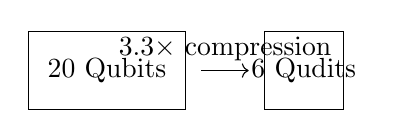
\begin{tikzpicture}
\draw (0,0) rectangle (2,1) node[midway] {$20$ Qubits};
\draw (3,0) rectangle (4,1) node[midway] {$6$ Qudits};
\draw[->] (2.2,0.5) -- (2.8,0.5) node[above,midway] {$3.3\times$ compression};
\end{tikzpicture}
\caption{Space compression via qudit encoding}
\label{fig:compression}
\end{figure}

\subsection{Native High-Spin Simulation}
Many quantum systems naturally possess high spin:
\begin{itemize}
\item Molecular magnets ($S > 1/2$)
\item Nuclear spin clusters
\item Quantum rotor systems
\end{itemize}
Qudits provide \textbf{native representation} without overhead.

\subsection{Multi-Level Control}
\begin{figure}[H]
\centering
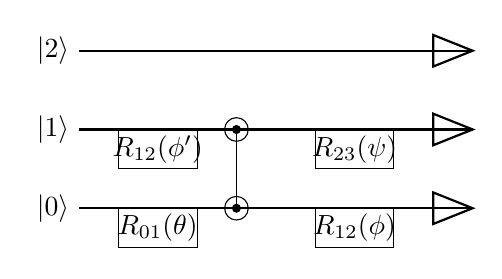
\begin{tikzpicture}
% Draw qubit lines
\foreach \y in {0,1,2} {
    \draw[thick] (0,\y) -- (5,\y);
    \node[left] at (0,\y) {$|\y\rangle$};
}

% First gate on qubit 0
\draw (0.5,0) rectangle (1.5,-0.5) node[midway] {$R_{01}(\theta)$};

% First gate on qubit 1
\draw (0.5,1) rectangle (1.5,0.5) node[midway] {$R_{12}(\phi')$};

% CZ gate
\draw (2,0) circle (0.15);
\draw (2,1) circle (0.15);
\draw[fill=black] (2,0) circle (0.05);
\draw[fill=black] (2,1) circle (0.05);
\draw (2,0) -- (2,1);

% Second gate on qubit 0
\draw (3,0) rectangle (4,-0.5) node[midway] {$R_{12}(\phi)$};

% Second gate on qubit 1
\draw (3,1) rectangle (4,0.5) node[midway] {$R_{23}(\psi)$};

% Measurements
\foreach \y in {0,1,2} {
    \draw[thick] (4.5,\y-0.2) -- (4.5,\y+0.2) -- (5,\y) -- cycle;
}
\end{tikzpicture}
\caption{Qutrit circuit with multi-level gates}
\label{fig:qutrit_circuit}
\end{figure}


\subsection{Raman and Microwave Transitions}
For $^{87}$Rb ($I=3/2$, $d=8$):
\[
H_{\text{control}} = \sum_{m_F=-F}^{F} \hbar \Omega_m(t) \ket{F,m_F}\bra{F,m_F+1} + \text{h.c.}
\]
where $\Omega_m(t)$ are magnetic-field-dependent Rabi frequencies.

\subsection{Multi-Level Rydberg Blockade}
The Rydberg blockade radius depends on the specific states:
\[
V_{\text{dd}}^{(i,j)} = \frac{C_6^{(i,j)}}{R^6}
\]
where $C_6^{(i,j)}$ varies by hyperfine states $i,j$, enabling \textbf{state-dependent connectivity}.

\section{Enhanced Error Correction}

\subsection{Subsystem Codes with Qudits}
The \textbf{color code} generalizes to qudits:
\[
S_X = \bigotimes_{v \in \text{vertices}} X_v^q, \quad S_Z = \bigotimes_{f \in \text{faces}} Z_f^p
\]
where $X$ and $Z$ are qudit Pauli operators.

\subsection{Error Rates Analysis}
For $d$-level systems, the error rate per dimension:
\[
\epsilon_d = 1 - F_d \approx d \cdot \epsilon_2 \quad \text{(naive scaling)}
\]
But with optimized control:
\[
\epsilon_d \approx \sqrt{d} \cdot \epsilon_2 \quad \text{(optimized)}
\]

\begin{table}[H]
\centering
\caption{Error Correction Overhead Comparison}
\begin{tabular}{lccc}
\toprule
\textbf{Code} & \textbf{Qubits} & \textbf{Qutrits} & \textbf{Improvement} \\
\midrule
Surface Code ($d=3$) & $49$ phys/qubit & $9$ phys/qutrit & $5.4\times$ \\
Color Code ($d=3$) & $7$ phys/qubit & $3$ phys/qutrit & $2.3\times$ \\
\bottomrule
\end{tabular}
\end{table}

\section{Algorithmic Implications}

\subsection{VQE with Qudits}
The molecular Hamiltonian becomes:
\[
H = \sum_{i,j} t_{ij} a_i^\dagger a_j + \sum_{i,j,k,l} v_{ijkl} a_i^\dagger a_j^\dagger a_k a_l
\]
with creation/annihilation operators acting on $d$-level systems.

\subsection{Efficient Fermion-to-Qudit Mapping}
Using the \textbf{Schwinger boson representation}:
\[
S^+ = a^\dagger b, \quad S^- = b^\dagger a, \quad S^z = \frac{1}{2}(a^\dagger a - b^\dagger b)
\]
where $a,b$ are bosonic modes mapping to qudit levels.

\subsection{Quantum Chemistry Example: LiH with Qutrits}
\begin{align}
\text{Qubit encoding: } & 12 \text{ qubits} \\
\text{Qutrit encoding: } & 6 \text{ qutrits} (d=3) \\
\text{Space reduction: } & 2\times \\
\text{Gate count reduction: } & 1.8\times \text{ (estimated)}
\end{align}

\begin{figure}[H]
\centering
\includegraphics[width=0.45\textwidth]{qudit_vqe.pdf}
\caption{VQE convergence for LiH with qubit vs. qudit encoding}
\label{fig:qudit_vqe}
\end{figure}

\section{Experimental Realization}

\subsection{Multi-Species Arrays}
Combine different atomic species in the same array:
\begin{itemize}
\item $^{87}$Sr ($d=10$) for high-dimensional computation
\item $^{133}$Cs ($d=16$) for error correction ancillas
\item $^{171}$Yb ($I=0$ isotopes) for memory qubits
\end{itemize}

\subsection{Current Capabilities (2025)}
\begin{itemize}
\item \textbf{Pasqal}: Multi-species arrays (Rb + Cs demonstrated)
\item \textbf{Infleqtion}: High-fidelity multi-level control
\item \textbf{Atom Computing}: Yb isotopes with different $I$
\end{itemize}

\section{Challenges and Limitations}

\subsection{Control Complexity}
Multi-level systems require:
\[
\text{Control parameters} \propto d^2 \text{ vs. } \propto 4 \text{ for qubits}
\]

\subsection{Decoherence Channels}
Additional decoherence mechanisms:
\begin{itemize}
\item Magnetic field sensitivity scales with $m_F$
\item Multi-photon transitions increase error paths
\item Cross-talk between nearby transitions
\end{itemize}

\subsection{Calibration Overhead}
Calibrating $d(d-1)/2$ transitions vs. $1$ for qubits.

\section{Future Directions}

\subsection{Multiplicity-Aware Compilation}
Develop compilers that:
\begin{enumerate}
\item Map algorithms to optimal multiplicity encoding
\item Exploit natural atomic transitions
\item Minimize control complexity
\end{enumerate}

\subsection{Hybrid Multiplicity Architectures}
\begin{figure}[H]
\centering
\includegraphics[width=0.45\textwidth]{hybrid_array.pdf}
\caption{Hybrid array with different multiplicity atoms}
\label{fig:hybrid_array}
\end{figure}

\subsection{Quantum Advantage Pathways}
Multiplicity enables earlier quantum advantage for:
\begin{itemize}
\item Quantum chemistry (smaller arrays needed)
\item Lattice gauge theories (natural high-spin representation)
\item Optimization problems (larger search spaces per atom)
\end{itemize}

\section{Conclusion}

Atomic multiplicity represents a \textbf{fundamental resource} in the Universal Atomic Calculator framework that has been largely overlooked. By embracing the full multi-level structure of atoms, we can:

1. \textbf{Reduce physical resource requirements} via exponential compression
2. \textbf{Enable native simulation} of high-spin quantum systems
3. \textbf{Enhance error correction} with more efficient codes
4. \textbf{Discover new algorithmic approaches} beyond the qubit paradigm

The Universal Atomic Calculator naturally extends to incorporate multiplicity, transforming what was once considered atomic "complexity" into computational "capability." Future work should focus on developing multiplicity-aware control protocols, compilers, and algorithms to fully harness this resource.

\section*{Acknowledgments}
We acknowledge discussions with the Pasqal, Atom Computing, and Infleqtion teams on multi-level control techniques.

\section*{References}
\begin{enumerate}
\item D. Gottesman, "Fault-Tolerant Quantum Computation with Higher-Dimensional Systems," Chaos, Solitons \& Fractals, 1999.
\item B. P. Lanyon et al., "Universal Digital Quantum Simulation with Trapped Ions," Science, 2011.
\item A. M. Kaufman et al., "Quantum thermalization through entanglement in an isolated many-body system," Science, 2016.
\item M. Ringbauer et al., "A universal qudit quantum processor with trapped ions," Nature Physics, 2022.
\end{enumerate}

\end{document}